\documentclass[../main.tex]{subfiles}

\begin{document}
Now that we have familiarized ourselves with the way a parallel RLC resonator
behaves and how we can optimize it for the best possible contrast, we are going
to analyze how the inclusion of a variable \(L\) via a kinetic inductor
will affect the contrast of our circuit.

% \begin{figure}
% \centering
% \begin{circuitikz}[]
%     \draw (-0.5,0) to[short]
%           (0,0) to[generic, l=\(Z_0\)]
%           (1.5,0) to[capacitor, l=\(C_c\)]
%           (3,0) to[short]
%           (6,0);
%     \draw (3,0) to[vL, l=\(L\)]
%           (3,-1.5);
%     \draw (0,-1.5) to[R, l=\(R_{DC}\)]
%           (3,-1.5) to [short]
%           (3,-1.7) to[capacitor]
%           (3,-2) node[ground]{};
%     \draw (4.5,0) to[capacitor, l=\(C_p\)]
%           (4.5,-2);
%     \draw (6,0) to[vR, l=\({R = R_{SET} \parallel R_p}\)]
%           (6,-2);
%     \draw (4.5,-2) to[short]
%           (6,-2) node[ground]{};
% \end{circuitikz}
% \caption{Modified circuit for a kinetic inductor. Since \(C_{p}\) and \(R_{p}\)
% are virtual components added to model losses in the circuit, the direct current
% that passes }
% \label{fig:KineticRLC}
% \end{figure}

Like with the resistance, the measure of the qubit in the state \(1\) will be
linked with an inductance \(\LOn\), and an inductance
\(\LOff\) with the state \(0\). Taking a page out of the previous
section, we are going to introduce a parameter \(\lambda\) defined as
\begin{equation}
\label{eq:LambdaDef}
    \lambda = \frac{\LOff}{\LOn}
\end{equation}
It's important to denato that \(0 < \lambda \leq 1\), unlike \(\rho\). This is due to
\(\ROn < \ROff\) and that the voltage is constant, so
\(I_{\text{On}} > I_{\text{Off}}\).

One more thing we need to cover before trying to get a usable expression for
the optimum contrast is a new problem that comes with a variable inductance:
which one do we use? Since we don't know which one is best, we'll introduce
the parameter \(1 \leq \lambda_{t} \leq \lambda\) such that
\(\omega = \frac{1}{\sqrt{\lambda_{t}\LOn(C_{c} + C_{p})}}\).
This parameter will determine the tuning we will be using, which will boil
down to 3:

\begin{itemize}[]
    \item \(\LOn\) tuning (\(\lambda_{t} = 1\))
    \item \(\LOff\) tuning (\(\lambda_{t} = \lambda\))
    \item Middle tuning (\(1 < \lambda_{t} < \lambda\))
\end{itemize}

We won't consider the outside of this interval of frequencies because as we
shall see it's objectively worse than any of these 3 options.

\subsection{Analysis of the effect on kinetic inductance on the contrast}
We start in the same way as in \ref{eq:ImpParallelResonant}: with the most generic
expression for the inductance and little by little we start to specify more
and more (for example, with an expression for \(\omega\)).

\begin{align}
\label{eq:ImpKineticResonant}
\begin{split}
    Z &= \frac{1}{j \omega(\lambda_{t}) C_{p} + \frac{1}{j \omega(\lambda_{t}) \lambda\LOn} + \frac{1}{R}}
        + \frac{1}{j \omega(\lambda_{t}) C_{c}}\\
      &= \frac{\omega(\lambda_{t}) R \lambda\LOn}{R(1 - \omega(\lambda_{t})^2 \lambda\LOn C_{p}) + j \omega(\lambda_{t}) \lambda\LOn}
        + \frac{1}{j \omega(\lambda_{t}) C_{c}}\\
      &= \frac{R \lambda\LOn}{\frac{R}{\omega(\lambda_{t})}(1 - \omega(\lambda_{t})^2 \lambda\LOn C_{p}) + j \lambda\LOn}
        + \frac{1}{j \omega(\lambda_{t}) C_{c}}\\
      &= \frac{j R \lambda\LOn}{
          \frac{R\omega(\lambda_{t})}{\omega(\lambda_{t})^2}\left(1 - \frac{\lambda\cancel{\LOn} C_{p}}{\lambda_{t}\cancel{\LOn}(C_{c} + C_{p})}\right)
            + j \lambda\LOn} + \frac{1}{j \omega(\lambda_{t})C_{c}}\\
      &= \frac{j R \lambda\LOn}{
          R\omega(\lambda_{t})\cancel{\lambda_{t}}\LOn\cancel{(C_{c} + C_{p})}
          \left(\frac{\lambda_{t}(C_{c} + C_{p}) - \lambda C_{p}}{\cancel{\lambda_{t}}\cancel{(C_{c} + C_{p})}}\right)
            + j \lambda\LOn} + \frac{1}{j \omega(\lambda_{t})C_{c}}\\
      &= \frac{j R \cancel{\lambda}\cancel{\LOn}}{
          R\omega(\lambda_{t})\cancel{\LOn}\cancel{\lambda}
          \left(\frac{\lambda_{t}}{\lambda}(C_{c} + C_{p}) - C_{p}\right)
          + j \cancel{\lambda}\cancel{\LOn}} + \frac{1}{j \omega(\lambda_{t})C_{c}}\\
      &= \frac{j R }{
          R\omega(\lambda_{t})
          \left(\frac{\lambda_{t}}{\lambda}(C_{c} + C_{p}) - C_{p}\right)
          + j } + \frac{1}{j \omega(\lambda_{t})C_{c}}\\
\end{split}
\end{align}

As you can see, since the inductance of \(Z\) interacts with the one inside
\(\omega\), I've written directly \(\lambda\LOn\) instead of \(L\) to then
swap it, like with \(R\). So to get \(Z_{\text{On}}\) the substitutions needed
are \(R = \ROn\) and \(\lambda = 1\), and for \(Z_{\text{Off}}\) is
just \(\ROff\).

With that detail out of the way we can see that, as opposed to the previous section,
we can't wrap neatly \(C_{c}\), \(C_{p}\) and \(L\) in a parameter like \(S\).
Due to this, I believe that to obtain an expression like the one for the non-kinetic resonator it would be necessary to do an analysis on a case by case bases
with more context about the application to better choose the correct approximations,
if arriving at a nice and practical expression is even possible that is. Since
the objective of this master's thesis is a theoretical proof of concept for the
use of kinetic inductors to improve readout for silicon spin qubits, simulations
and their analysis will be the methodology used.

\subsection{Simulation of the effect on kinetic inductance on the contrast}
In a simulation you have supreme control over what is simulated, how is
simulated and what and how results are shown. A great deal of time was spent
deciding these things, and the final decisions and their reasoning are the following:

The main value we are going to calculate and graph is
\(\Delta\Gamma(Z_{0}, \rho, \ROn, C_{p}, \LOn, \lambda_{t}, \pi, C_{c}, \lambda)\).

Due to the high number of inputs, we need to fix some of them in order to analyze
in the best way possible how does \(\Delta\Gamma\) behave. Taking inspiration
from the non-kinetic case, in which for the optimum value of \(C_{c}\) the
only parameter that affected the contrast was \(\pi\), we will fix the following
variable with the following values

% First we remember that \(Z_{0}\) is the impedance of our transmission line (which has
% a standard value), \(\rho\) is the ratio between the resistances of the 2 states
% of the SET (\ref{eq:RhoDef}), \(\ROn\) is the resistance of the SET in the On
% state, \(C_{p}\) is a parasitic capacitance used to model losses in the circuit,
% \(\LOn\) is the inductance of the kinetic inductor when  the state of the
% SET is On, \(\lambda_{t}\) is the parameter that determines what inductance
% to use to obtain the frequency of operation with respect to \(\LOn\),
% \(\pi\) is the ratio between \(R_{p}\), a virtual resistance used to model
% losses in the circuit, and \(\ROn\) (\ref{eq:PiDef}), \(C_{c}\) is the control
% capacitance and \(\lambda\) is the ratio between the inductance in each state
% of the SET (\ref{eq:LambdaDef}).

\begin{table}[H]
    \centering
    \begin{tabular}{c|c|c|c|c}
        \(Z_{0}\) & \(\rho\) & \(\ROn\) & \(C_{p}\) & \(\LOn\) \\\hline
        \(50\unit{\ohm}\) & \(2\cdot10^{6}\) & \(50\unit{\kilo\ohm}\) & \(500\unit{\femto\farad}\) & \(180\unit{\nano\henry}\)
    \end{tabular}
\end{table}

So, what we will graph is \(\Delta\Gamma(\lambda_{t}, \pi, C_{c}, \lambda)\),
which only depends on \(\pi\), \(C_{c}\) (since we'll need to find the optimal
value numerically), and all the new variables associated with the introduction
of a variable inductance. This still leaves us with a 4 variable function, and
the best way to plot it that I could think of can be seen in figure
\ref{fig:IdealContrast}

\begin{figure}[t]
\centering
  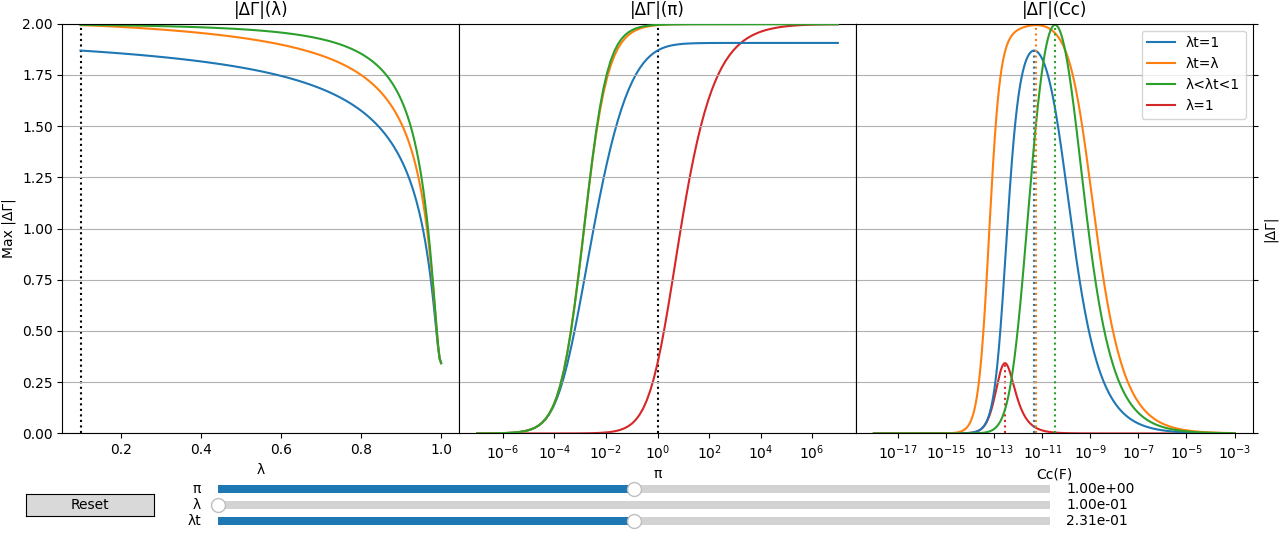
\includegraphics[width=\linewidth]{RLCKinetic/IdealContrastOfRp&Lf&Cc.png}
  \caption{Multiple representations of the contrast with sliders to control
  their parameters. Right: \(|\Delta\Gamma_{\text{Opt}}(\lambda)|\).
  Center \(|\Delta\Gamma_{\text{Opt}}(\pi)|\). Left: \(|\Delta\Gamma(C_{c})|\)}
\label{fig:IdealContrast}
\end{figure}

In the left and central plot we have the modulus of \(\Delta\Gamma_{\text{Opt}}\),
which is \(\Delta\Gamma\) with the value of \(C_{c}\) that maximizes the modulus,
as a function of \(\lambda\) and \(\pi\) respectively, and the left plot
is \(|\Delta\Gamma(C_{c}|\). In each there are multiple lines: 3 with a different
value of \(\lambda_{t}\) and one with \(\lambda = 1\) to act as reference for
the non-kinetic case (for the left plot it didn't make sense to add the reference
line). Finally, we have 3 sliders to control the plots in real time:

\begin{itemize}
    \item \(\pi\) slider controls the value of \(\pi\) for the left and right
        plot, and the dotted black line in the center plot
    \item \(\lambda\) slider controls the value of \(\lambda\) for the center
        and right plot, and the dotted black line in the left plot
    \item \(\lambda_{t}\) slider controls the value of \(\lambda_{t}\) for
        the plot with \(\lambda < \lambda_{t} < 1\)
\end{itemize}

The range of the \(\lambda\) and \(\pi\) sliders is the same as the domain
of the respective plots (\(\lambda \in [0.1, 1]\), \(\pi \in [10^{-7}, 10^{7}]\)),
and the range of the \(\lambda_{t}\) slider is \(\lambda_{t} \in [\lambda, 1]\)
(the edges were included, so it could be seen how it morphs into the other two plots).
The domain of the right plot is \(C_{c} \in [10^{-18}, 10^{-3}]\unit{\fF}\), and it
was chosen such that for any combination of \(\lambda\) and \(\pi\) the maxima
was in it, since it is also the range in which the simulation search for the
optimum \(C_{c}\).

The main observations, both in relevance and notoriety, can be seen directly
with figure \ref{fig:IdealContrast}
\begin{itemize}
    \item A smaller \(\lambda\) is always better in order to improve the contrast
    \item \(\lambda_{t}\) and \(\lambda < \lambda_{t} < 1\) are objectively better
        than the non-kinetic case, with the main difference being that with an
        intermediate \(\lambda_{t}\) the optimum \(C_{c}\) is greater
    \item \(\lambda_{t} = 1\) hits a ceiling that causes that, for a high enough
        value of \(\pi\), the introduction of a kinetic inductor is actually worse
        than a non-kinetic one. With the \(\pi\) slider can be seen that this
        ceiling depends on \(\lambda\), but modifying the non-variable parameters
        shows that it also depends on them. To be more specific,
        \(|\Delta\Gamma(\lambda_{t} = 1)|\propto \ROn, C_{p}, 1/\LOn\),
        with \(\ROn\) being the more sensible of the 3 by a margin.
\end{itemize}

Thanks to the sliders a more thorough analysis of the simulation can be made,
but nothing besides the previous points can be seen except for some
quirky behavior not drastic enough to necessitate images, but curious enough
to talk about it and encourage playing with the simulation to see it.

This behavior boils down to 3 quirks that appear on the plots, one for each, at
high enough values of \(\pi\). These oddities are, from left to right

\begin{itemize}
    \item A local minimum appears in the left plot on all lines as early as
        \(\pi = 3.09\) near \(\lambda = 1\)
    \item At \(\pi \approx 1526\), the central plot with \(\lambda_{t} = \lambda\)
        gets a sudden but small jump, caused by the next point in the list
    \item A second local maximum appears in the right plot with
        \(\lambda_{t} = \lambda\), and at \(\pi \approx 1526\) it surpasses the
        previous global maximum
\end{itemize}

\begin{figure}[t]
\centering
  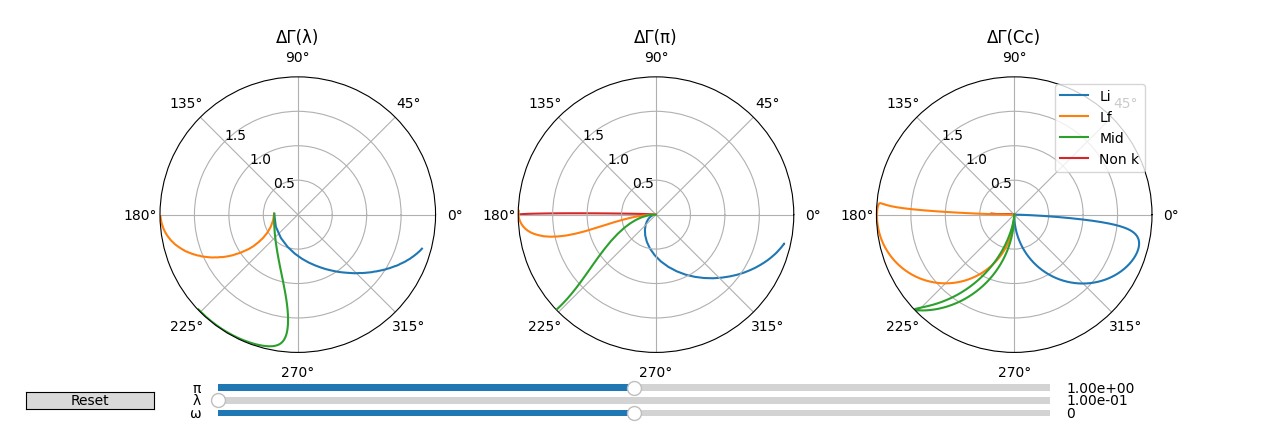
\includegraphics[width=\linewidth]{RLCKinetic/IdealComplexContrastOfRp&Lf&Cc.png}
  \caption{Multiple representations of the contrast with sliders to control
  their parameters. Right: \(\Delta\Gamma_{\text{Opt}}(\lambda)\).
  Center \(\Delta\Gamma_{\text{Opt}}(\pi)\). Left: \(\Delta\Gamma(C_{c})\)}
\label{fig:IdealComplexContrast}
\end{figure}

We can easily find an explanation by looking at \(\Delta\Gamma\) instead of
\(|\Delta\Gamma|\). When increasing \(\pi\), the origin of the lines in the
left plot of figure \ref{fig:IdealComplexContrast} shifts to the left, while
the ends stay relatively similar, making the path curve to the center of the
complex plane. Similarly, the closed path with \(\lambda_{t} = \lambda\)
in the right plot crosser over itself at \(\pi \approx 66\), causing the
second maximum to appear and at \(\pi \approx 1526\), it surpasses the previous
and causes the sudden rise in \(|\Delta\Gamma(\pi)|\).

\end{document}
